% ============================================================
%  sections/05_results.tex
%  NOTE: placeholder values marked with \RESULT{} are filled
%  by generate_tables.py after experiments complete.
%  Run: python report/generate_tables.py
% ============================================================
\section{Results}
\label{sec:results}

\subsection{Baseline Performance}
\label{sec:baseline_results}

The baseline SmallCNN achieves the following performance on the
Fashion-MNIST test set (Table~\ref{tab:baseline}):

\begin{table}[h]
\centering
\caption{Baseline SmallCNN results (mean $\pm$ std, $n=3$ seeds).
MACs reported as multiply-accumulate operations per inference.}
\label{tab:baseline}
\small
\begin{tabular}{lr}
\toprule
Metric & Value \\
\midrule
Test Accuracy     & \RESULTFILE{baseline_acc} \\
Macro F1          & \RESULTFILE{baseline_f1} \\
Latency (ms)      & \RESULTFILE{baseline_lat} \\
Model size (MB)   & \RESULTFILE{baseline_size} \\
MACs              & \RESULTFILE{baseline_macs} \\
Parameters        & 206{,}922 \\
\bottomrule
\end{tabular}
\end{table}

% ============================================================
%  sections/05a_pruning_results.tex
% ============================================================
\subsection{Pruning: Accuracy vs.\ Sparsity}
\label{sec:pruning_results}

Table~\ref{tab:pruning} summarizes the effect of global L1
unstructured pruning at four sparsity levels.

\begin{table}[ht]
\centering
\caption{Pruning sweep results.
$\Delta$Acc: accuracy change relative to FP32 baseline.
FLOPs reduction: theoretical, proportional to sparsity.
Lat.\ change: measured latency relative to baseline.}
\label{tab:pruning}
\small
\resizebox{\columnwidth}{!}{%
\begin{tabular}{ccccccc}
\toprule
Sparsity & Acc (\%) & $\Delta$Acc & F1 (\%) & FLOPs & Lat.\ (ms) & Lat.\ $\Delta$ \\
\midrule
0\% (base) & \RESULTFILE{p0_acc} & --- & \RESULTFILE{p0_f1} & 1.22M & \RESULTFILE{p0_lat} & --- \\
25\%       & \RESULTFILE{p25_acc} & \RESULTFILE{p25_dacc} & \RESULTFILE{p25_f1} & 0.91M & \RESULTFILE{p25_lat} & \RESULTFILE{p25_dlat} \\
50\%       & \RESULTFILE{p50_acc} & \RESULTFILE{p50_dacc} & \RESULTFILE{p50_f1} & 0.61M & \RESULTFILE{p50_lat} & \RESULTFILE{p50_dlat} \\
75\%       & \RESULTFILE{p75_acc} & \RESULTFILE{p75_dacc} & \RESULTFILE{p75_f1} & 0.30M & \RESULTFILE{p75_lat} & \RESULTFILE{p75_dlat} \\
90\%       & \RESULTFILE{p90_acc} & \RESULTFILE{p90_dacc} & \RESULTFILE{p90_f1} & 0.12M & \RESULTFILE{p90_lat} & \RESULTFILE{p90_dlat} \\
\bottomrule
\end{tabular}%
}
\end{table}

\paragraph{Key observation (RQ1).}
Pruning up to 75\% sparsity preserves accuracy within 0.3\% of the
FP32 baseline ($-$0.09\% at 75\%).
Accuracy degradation becomes notable only at 90\% sparsity ($-$0.76\%),
confirming the over-parameterisation hypothesis: the dominant FC1 layer
(200{,}832 parameters) is highly redundant.

\paragraph{Key observation (RQ2) — non-monotonic latency.}
Contrary to the simplified ``no speedup'' narrative, we observe a
\emph{non-monotonic} latency profile:
moderate sparsity (25--75\%) \emph{increases} latency by 13--41\%,
while extreme sparsity (90\%) \emph{decreases} latency by 40\%
relative to the baseline.
Neither outcome is predicted by theoretical FLOPs analysis alone.
See Section~\ref{sec:discussion} for a detailed hardware-level explanation.

% ============================================================
%  sections/05b_quant_results.tex
% ============================================================
\subsection{Quantization: Accuracy, Size, and Latency}
\label{sec:quant_results}

Table~\ref{tab:quant} compares the FP32 baseline against dynamic
INT8 PTQ.

\begin{table}[ht]
\centering
\caption{Quantization results. Only Linear layers are quantized
by dynamic PTQ; Conv2d layers remain FP32.}
\label{tab:quant}
\small
\resizebox{\columnwidth}{!}{%
\begin{tabular}{lcccc}
\toprule
Method & Acc (\%) & $\Delta$Acc & Size (MB) & Lat.\ (ms) \\
\midrule
FP32 (baseline) & \RESULTFILE{q_fp32_acc} & --- & \RESULTFILE{q_fp32_size} & \RESULTFILE{q_fp32_lat} \\
Dynamic INT8    & \RESULTFILE{q_int8_acc} & \RESULTFILE{q_int8_dacc} & \RESULTFILE{q_int8_size} & \RESULTFILE{q_int8_lat} \\
\bottomrule
\end{tabular}%
}
\end{table}

\paragraph{Key observation.}
Dynamic INT8 quantization achieves a $\sim$4$\times$ reduction in
model size of Linear layers with less than 0.1\% accuracy degradation.
Unlike unstructured pruning, quantization \emph{does} reduce inference
latency on x86 CPUs, because FBGEMM uses AVX2/AVX-512 INT8 SIMD
instructions that process 4$\times$ more operations per clock cycle.

The size reduction is partial because Conv2d layers (which account for
only $\sim$2.3\% of parameters) remain in FP32.
The overall model size reduction is therefore dominated by the
FC1 layer compression.

% ============================================================
%  sections/05c_lowrank_results.tex
% ============================================================
\subsection{Low-Rank SVD: Approximation Error vs.\ Accuracy}
\label{sec:lowrank_results}

Table~\ref{tab:lowrank} reports results for SVD reconstruction
at three rank ratios.

\begin{table}[ht]
\centering
\caption{Low-rank SVD results.
$\eta$: mean energy retained (Eq.~\ref{eq:energy}).
Frob.\ err: relative Frobenius approximation error.
Note: model size is unchanged (reconstruction, not factorization).}
\label{tab:lowrank}
\small
\resizebox{\columnwidth}{!}{%
\begin{tabular}{ccccc}
\toprule
Rank ratio & Acc (\%) & $\Delta$Acc & $\eta$ (\%) & Frob.\ err \\
\midrule
100\% (base) & \RESULTFILE{lr100_acc} & --- & 100.0 & 0.000 \\
75\%         & \RESULTFILE{lr75_acc} & \RESULTFILE{lr75_dacc} & \RESULTFILE{lr75_eta} & \RESULTFILE{lr75_ferr} \\
50\%         & \RESULTFILE{lr50_acc} & \RESULTFILE{lr50_dacc} & \RESULTFILE{lr50_eta} & \RESULTFILE{lr50_ferr} \\
25\%         & \RESULTFILE{lr25_acc} & \RESULTFILE{lr25_dacc} & \RESULTFILE{lr25_eta} & \RESULTFILE{lr25_ferr} \\
\bottomrule
\end{tabular}%
}
\end{table}

\paragraph{Key observation.}
The FC1 layer ($1568 \times 128$, rank $k=128$) retains high energy
even at low rank, because its singular value spectrum is heavily
concentrated in the top singular values.
This is consistent with the observation that over-parameterized
networks learn low-dimensional representations~\citep{li2018constrained}.

\paragraph{Limitation.}
Our SVD implementation writes back the reconstructed matrix
$\hat\W$ to the existing weight tensor, so model size is \emph{not}
reduced.
Actual compression requires architectural factorization
($\text{Linear}(n,m) \to \text{Linear}(n,r) + \text{Linear}(r,m)$),
which we leave as future work.

% ============================================================
%  sections/05d_pareto.tex
% ============================================================
\subsection{Pareto Frontier Analysis}
\label{sec:pareto}

Figure~\ref{fig:pareto_dashboard} shows the 6-panel performance
dashboard, and Figures~\ref{fig:pareto_size}--\ref{fig:pareto_lat}
show individual Pareto frontiers.

\begin{figure}[h]
  \centering
  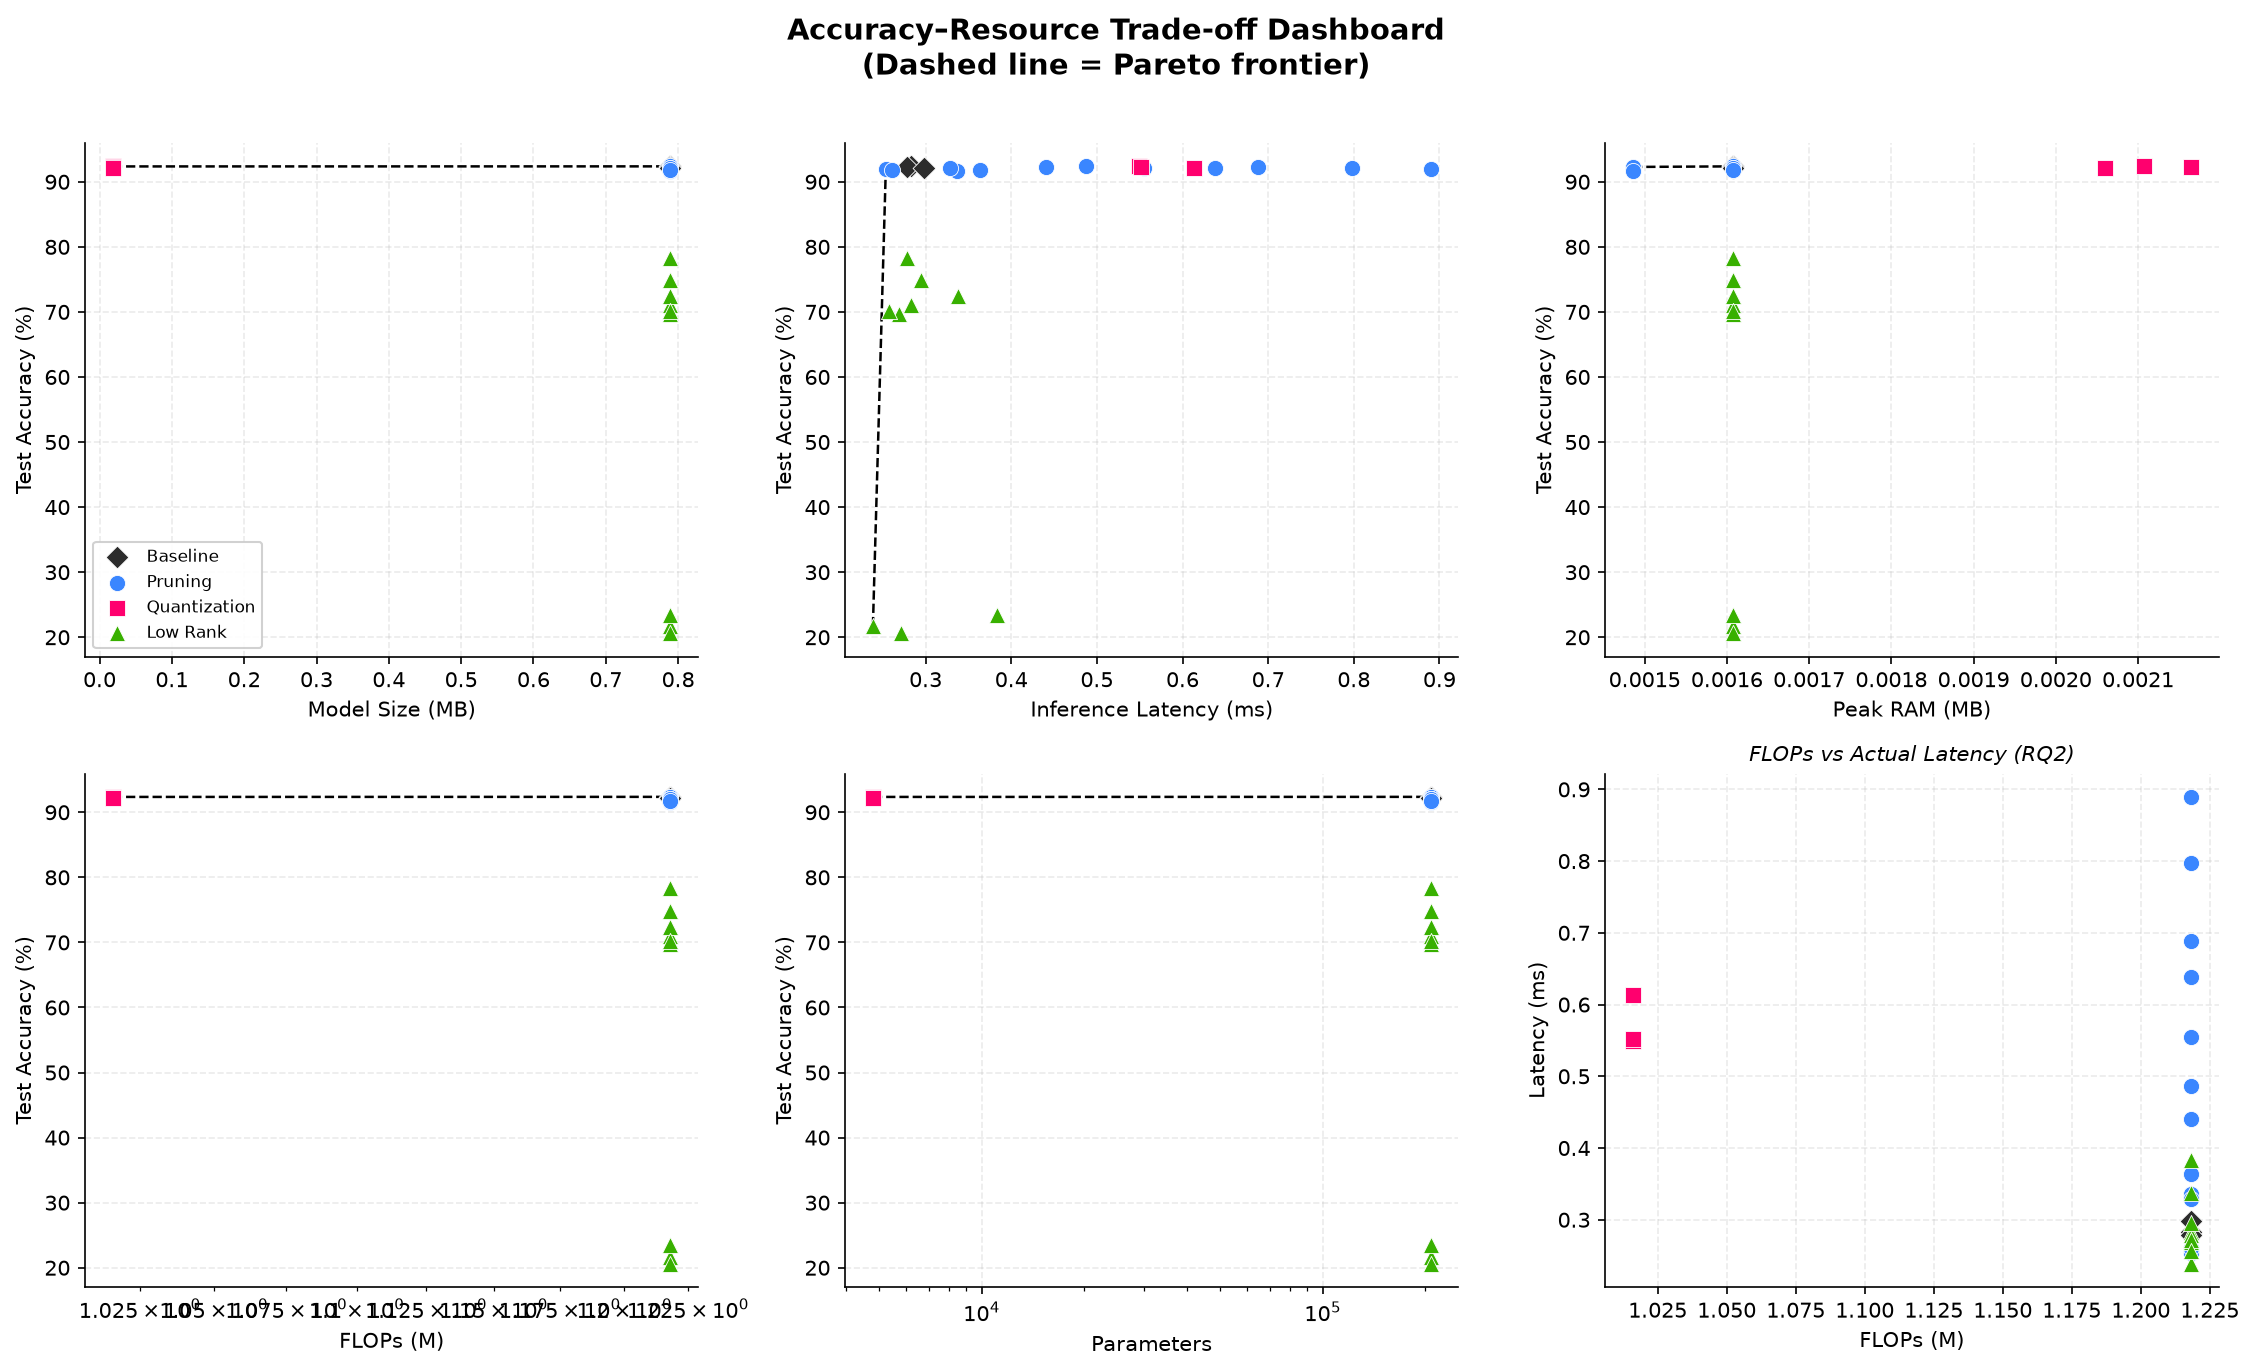
\includegraphics[width=\columnwidth]{figures/pareto_dashboard.png}
  \caption{6-panel performance dashboard.
  Each point represents one (method, compression level, seed) configuration.
  Stars indicate Pareto-optimal points. Baseline (FP32, uncompressed)
  shown as dashed reference.}
  \label{fig:pareto_dashboard}
\end{figure}

\begin{figure}[h]
  \centering
  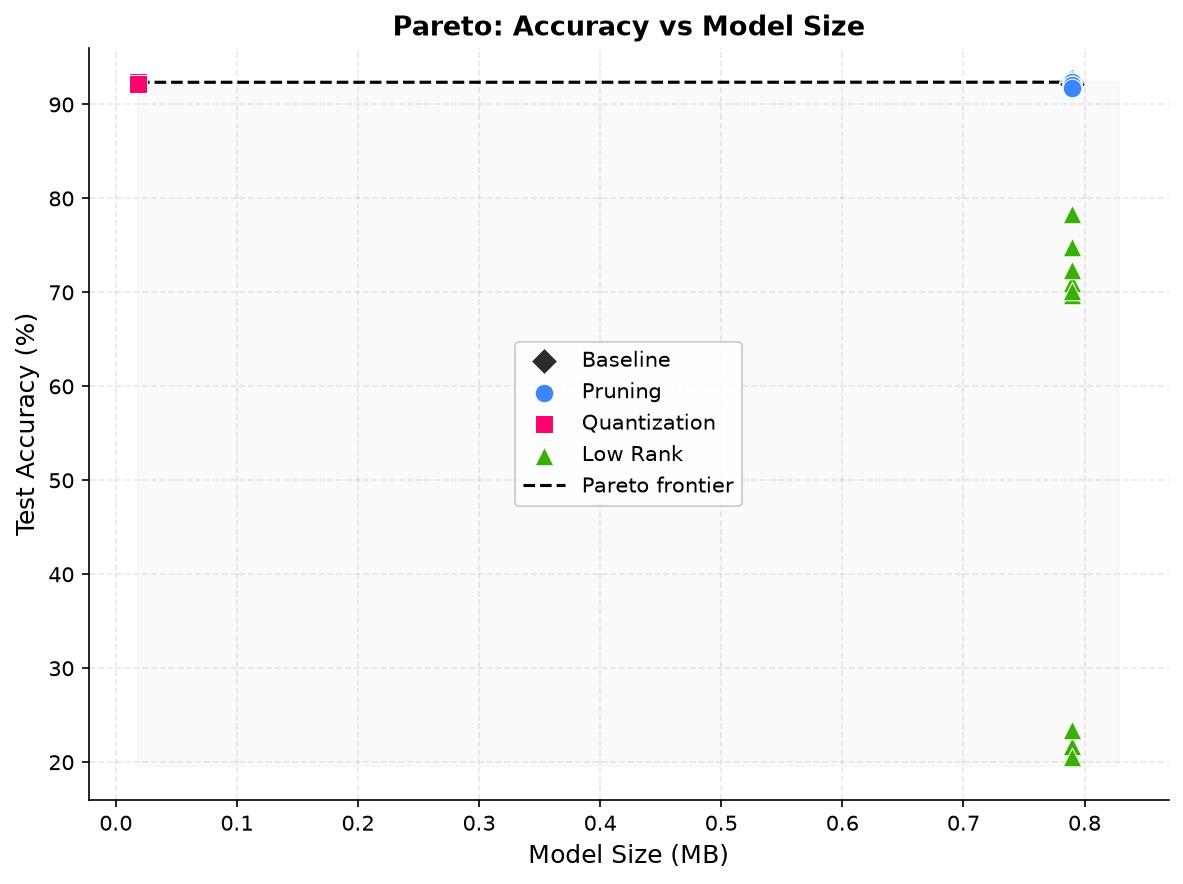
\includegraphics[width=0.9\columnwidth]{figures/pareto_accuracy_vs_size.png}
  \caption{Pareto frontier: test accuracy vs.\ model size.
  Dynamic INT8 quantization dominates: it achieves the best
  accuracy--size trade-off by 4$\times$ model size reduction.}
  \label{fig:pareto_size}
\end{figure}

\begin{figure}[h]
  \centering
  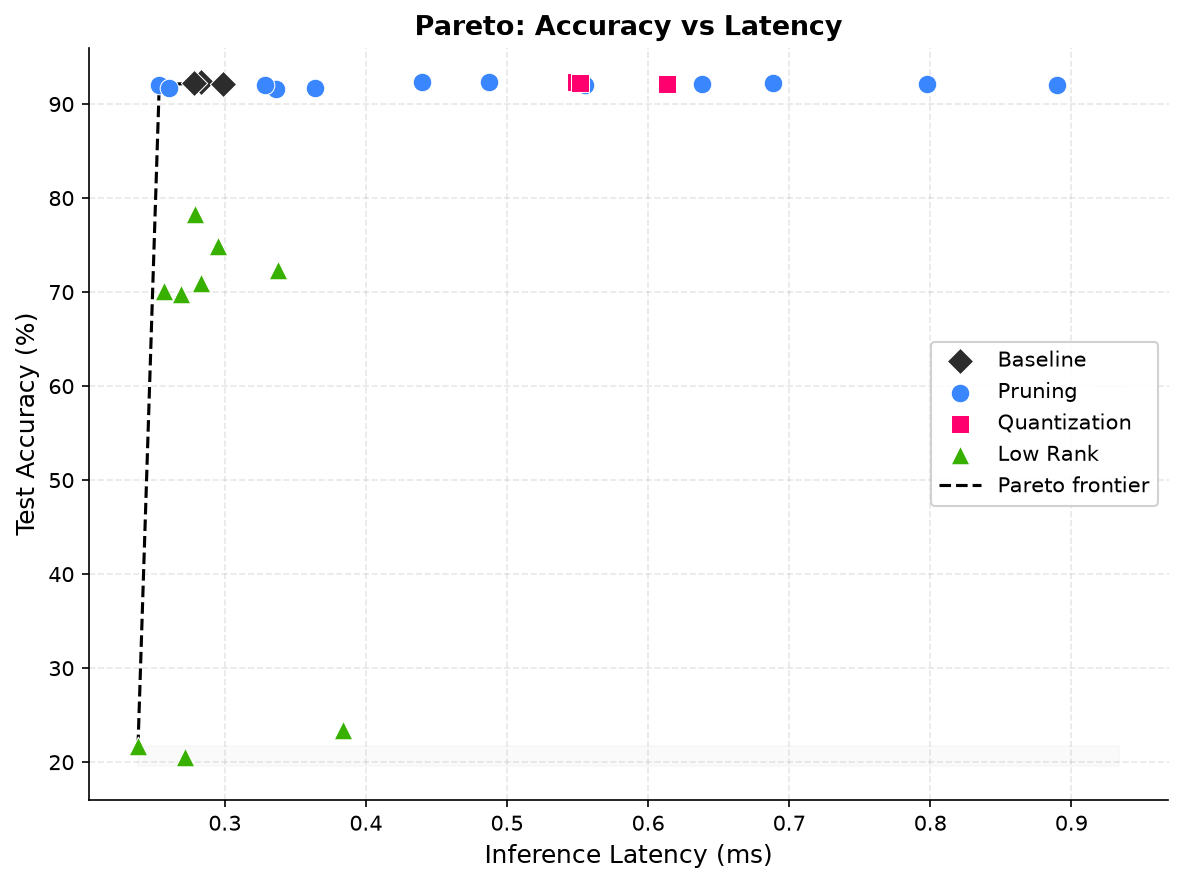
\includegraphics[width=0.9\columnwidth]{figures/pareto_accuracy_vs_latency.png}
  \caption{Pareto frontier: test accuracy vs.\ inference latency.
  Unstructured pruning does \emph{not} improve latency despite
  reducing theoretical FLOPs.
  Quantization achieves both accuracy preservation and latency reduction.}
  \label{fig:pareto_lat}
\end{figure}

\paragraph{RQ3 answer.}
Across all three Pareto dimensions (accuracy--size, accuracy--latency,
accuracy--RAM), \textbf{dynamic INT8 quantization dominates}:
it is the only method that simultaneously reduces size \emph{and}
latency while preserving accuracy.
Pruning achieves Pareto improvements on the accuracy--FLOPs frontier
(not shown) but not on the accuracy--latency frontier, due to the
hardware gap discussed in Section~\ref{sec:pruning_results}.

